\subsection{Analysing the results}



\begin{figure}[H]
    \makebox[\textwidth]{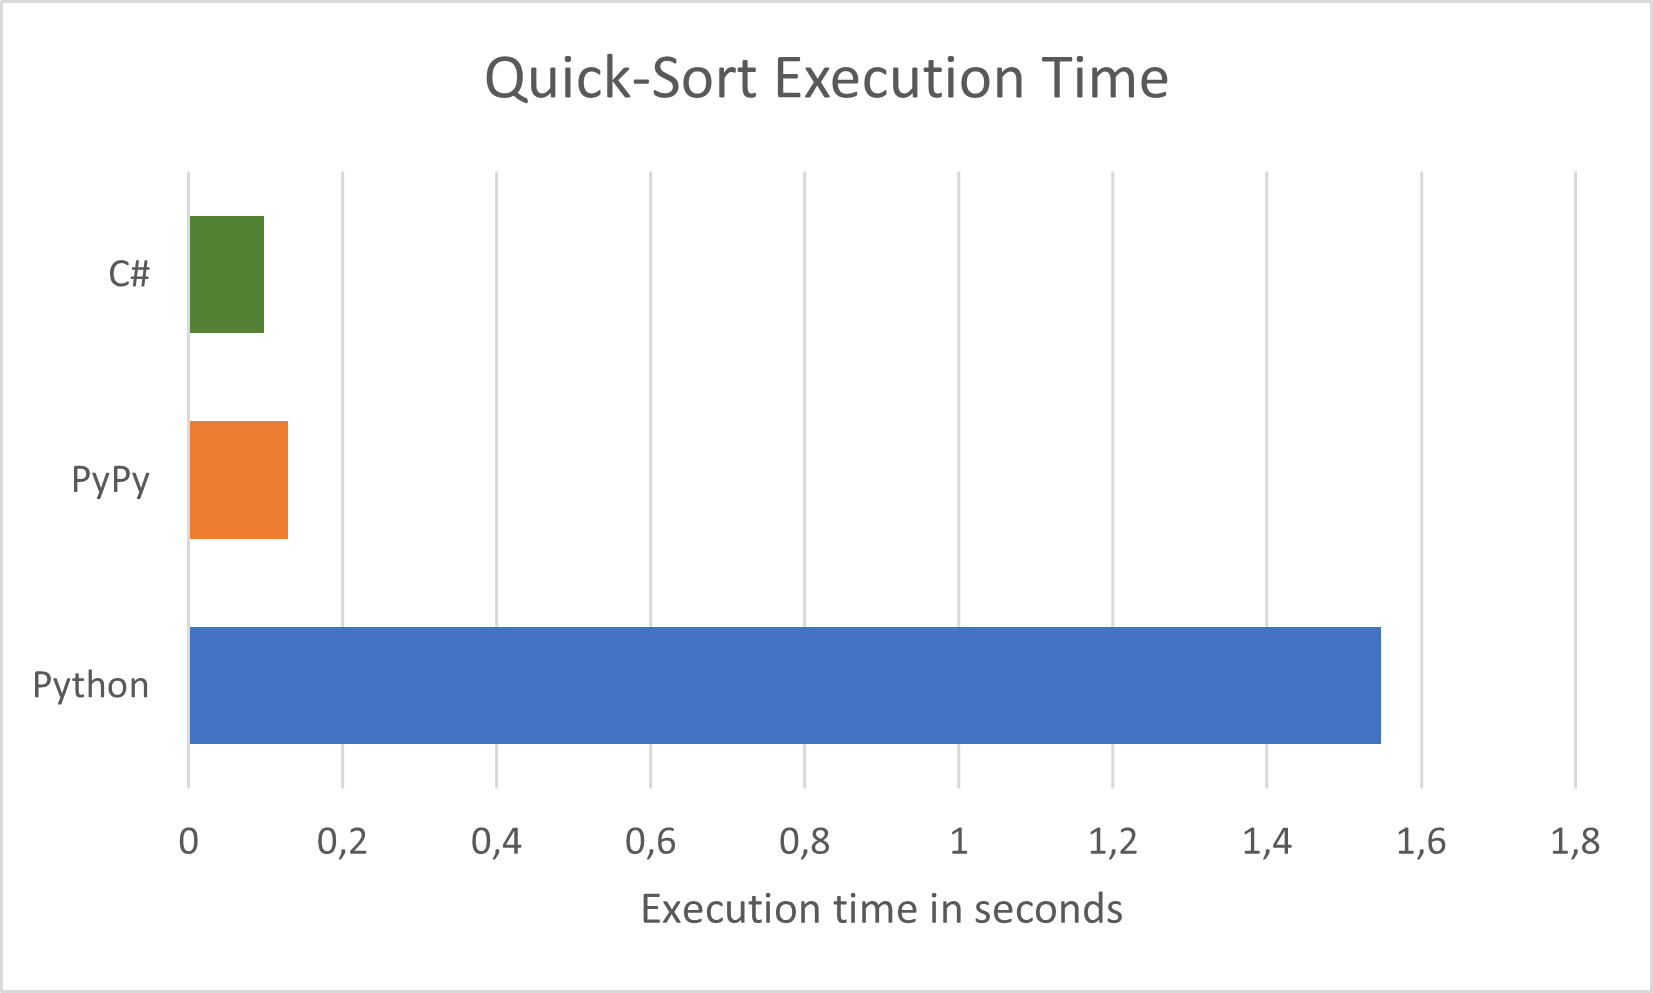
\includegraphics{src/images/qs_time_chart.png}}
    \vspace*{-0.8cm}
    \caption{A column chart that illustrates the difference in execution time}
\end{figure}

In the above diagram you can see the significant difference in execution time. You might wonder why PyPy is not standard if it's so much faster then native Python. The reason for this is that PyPy isn't supported by many of the popular packages, such as Pandas, SciPy and Matplotlib.\cite{quora_pypy}.

\begin{figure}[H]
    \makebox[\textwidth]{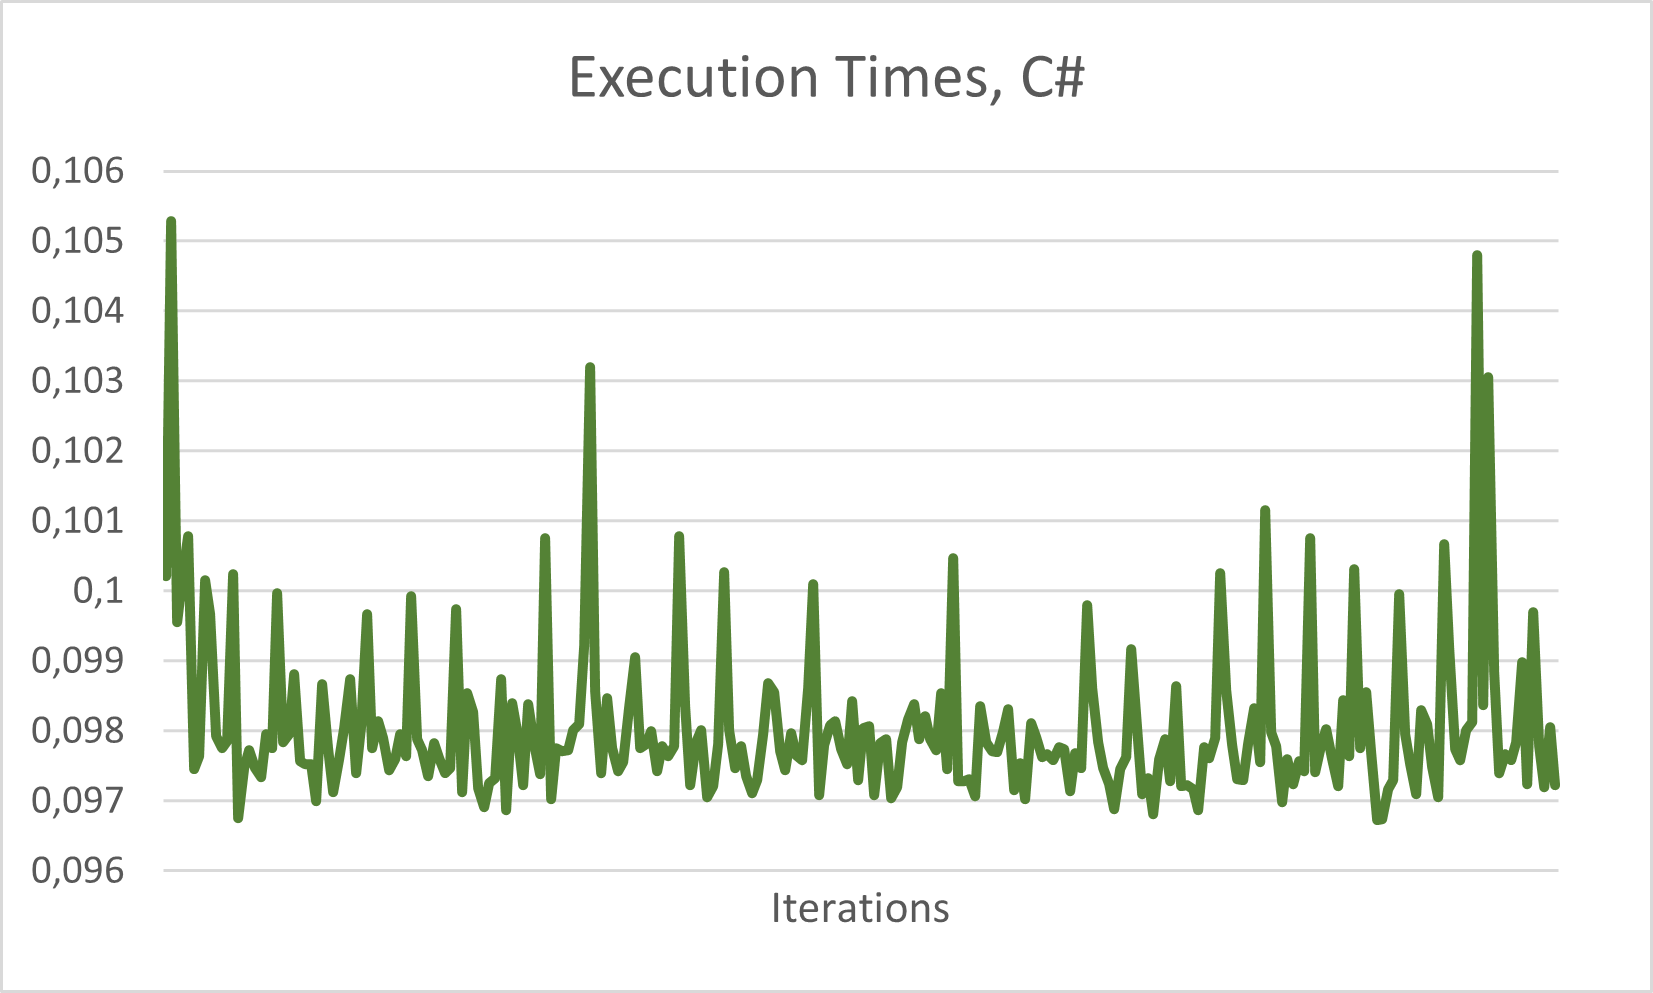
\includegraphics{src/images/qs_exe_time_csharp.png}}
    \vspace*{-0.8cm}
    \caption{A diagram that illustrates the different execution times for each iteration, in C\# for the small text file.}
\end{figure}

\noindent These results are more or less understandable. However, the spikes now and then boggles me. It could have something to do with a background program running on my PC. However the high spike at the beginning and the lower execution times throughout the iterations, are caused by the JIT compiler.

\begin{figure}[H]
    \makebox[\textwidth]{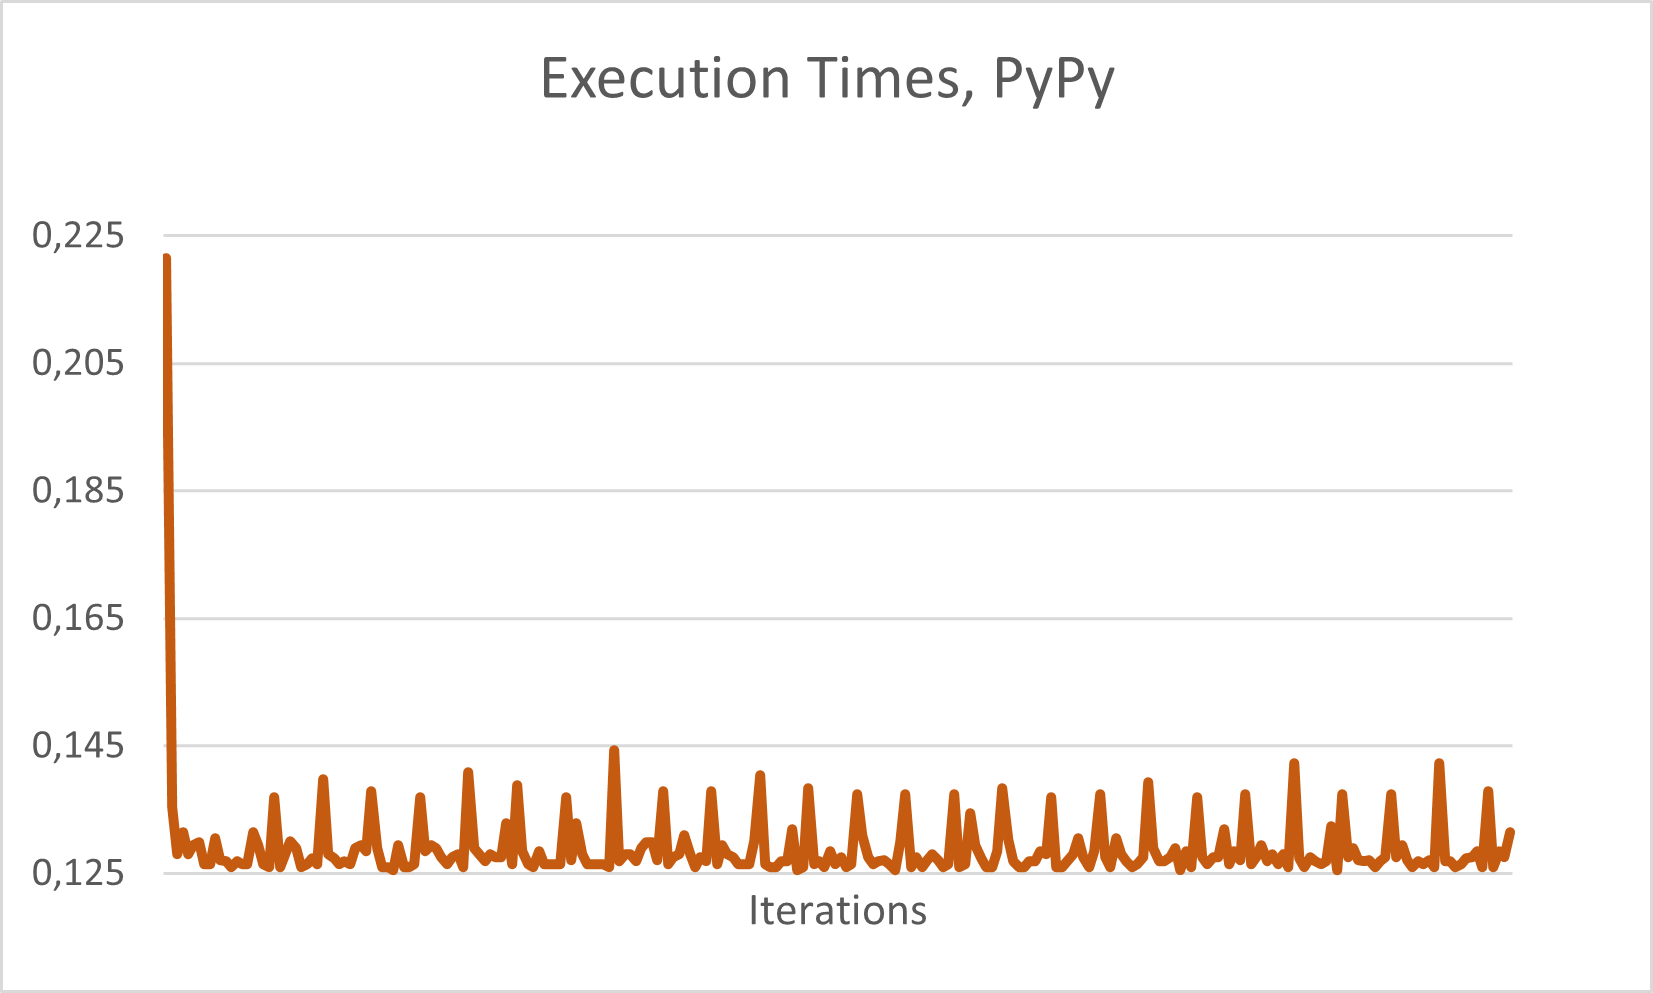
\includegraphics{src/images/qs_exe_time_pypy.png}}
    \vspace*{-0.8cm}
    \caption{A diagram that illustrates the different execution times for each iteration, in PyPY for the small text file.}
\end{figure}

\noindent Here we can see the JIT compiler at work. This is more along the lines, of what i expected from the execution times in C\#.

\begin{figure}[H]
    \makebox[\textwidth]{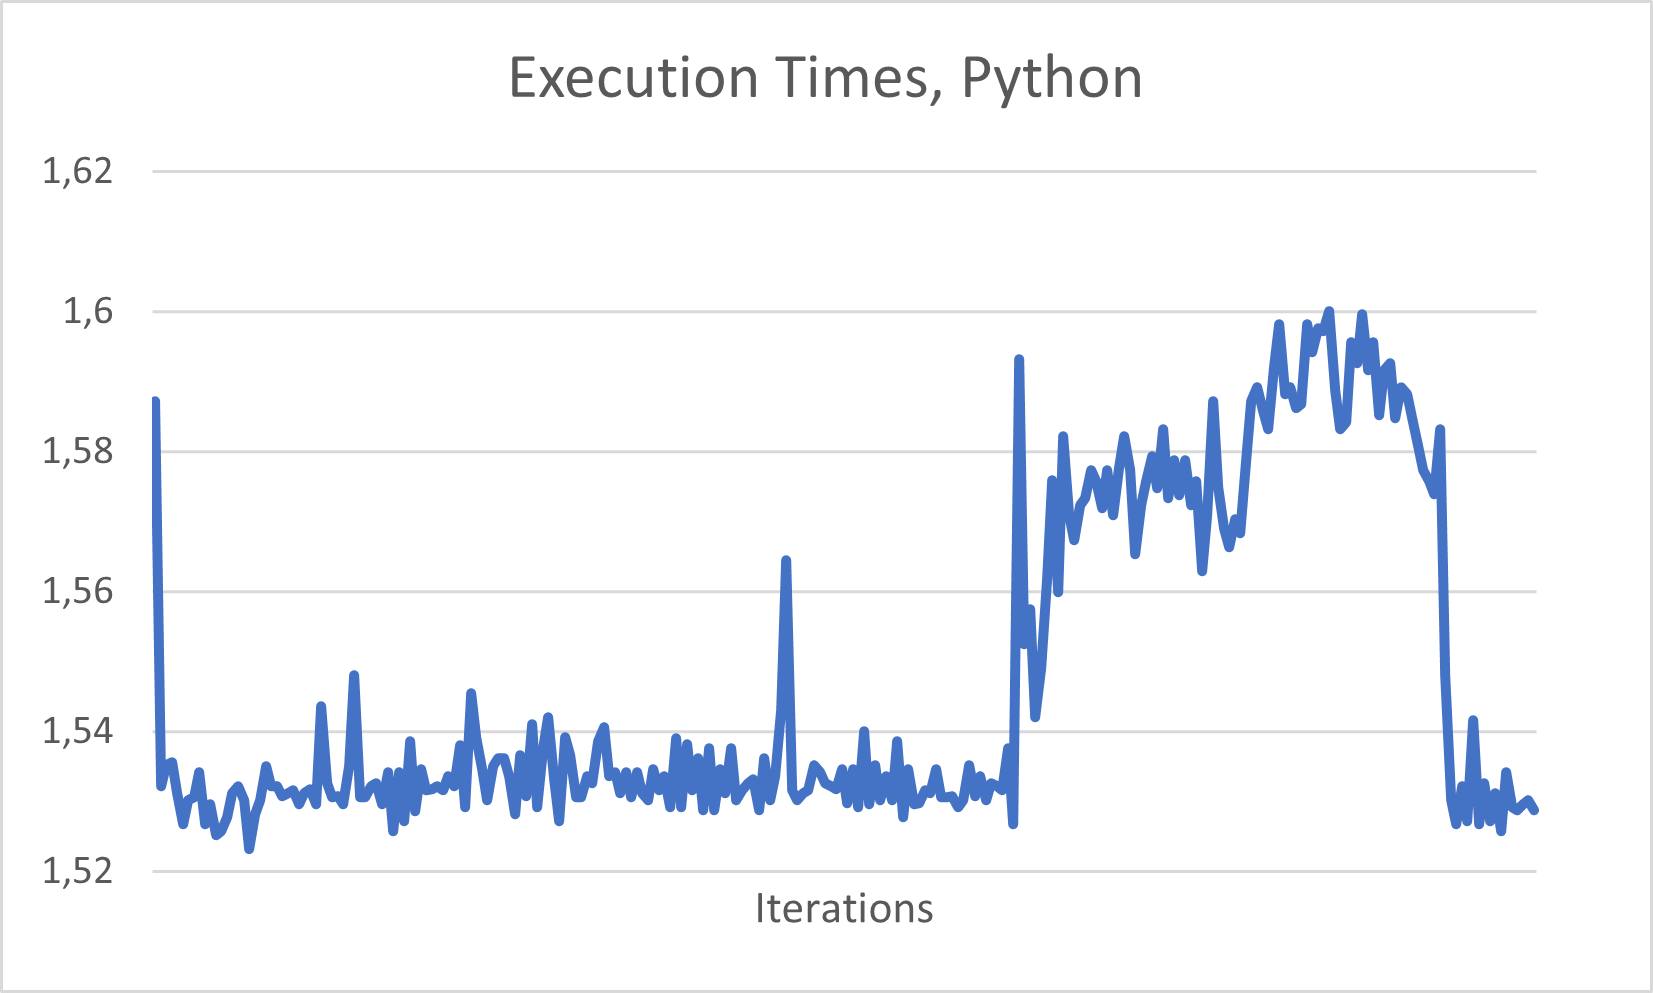
\includegraphics{src/images/qs_exe_time_python.png}}
    \vspace*{-0.8cm}
    \caption{A diagram that illustrates the different execution times for each iteration, in Python for the small text file.}
\end{figure}

\noindent The last group of executions times must have something to do with a background-program updating on my PC. Nonetheless it doesn't effect the comparison much. Since it would still have a way higher, minimum and maximum execution time.